% ================= Appendix A =================
\chapter{Field Consultation with NSL Experts}
\label{app:fieldwork}

The signed form of each of the six emergency phrases was established in person with Deaf experts before any data collection began, as described in Section~\ref{sec:phase0}. Consultations were held at the Rehabilitation Centre for the Rural Deaf in Bhaktapur and at the National Federation of the Deaf Nepal in Ranibari Marga, Samakhushi, Kathmandu. The images below are reproduced with the consent of those photographed.

\begin{figure}[H]
    \centering
    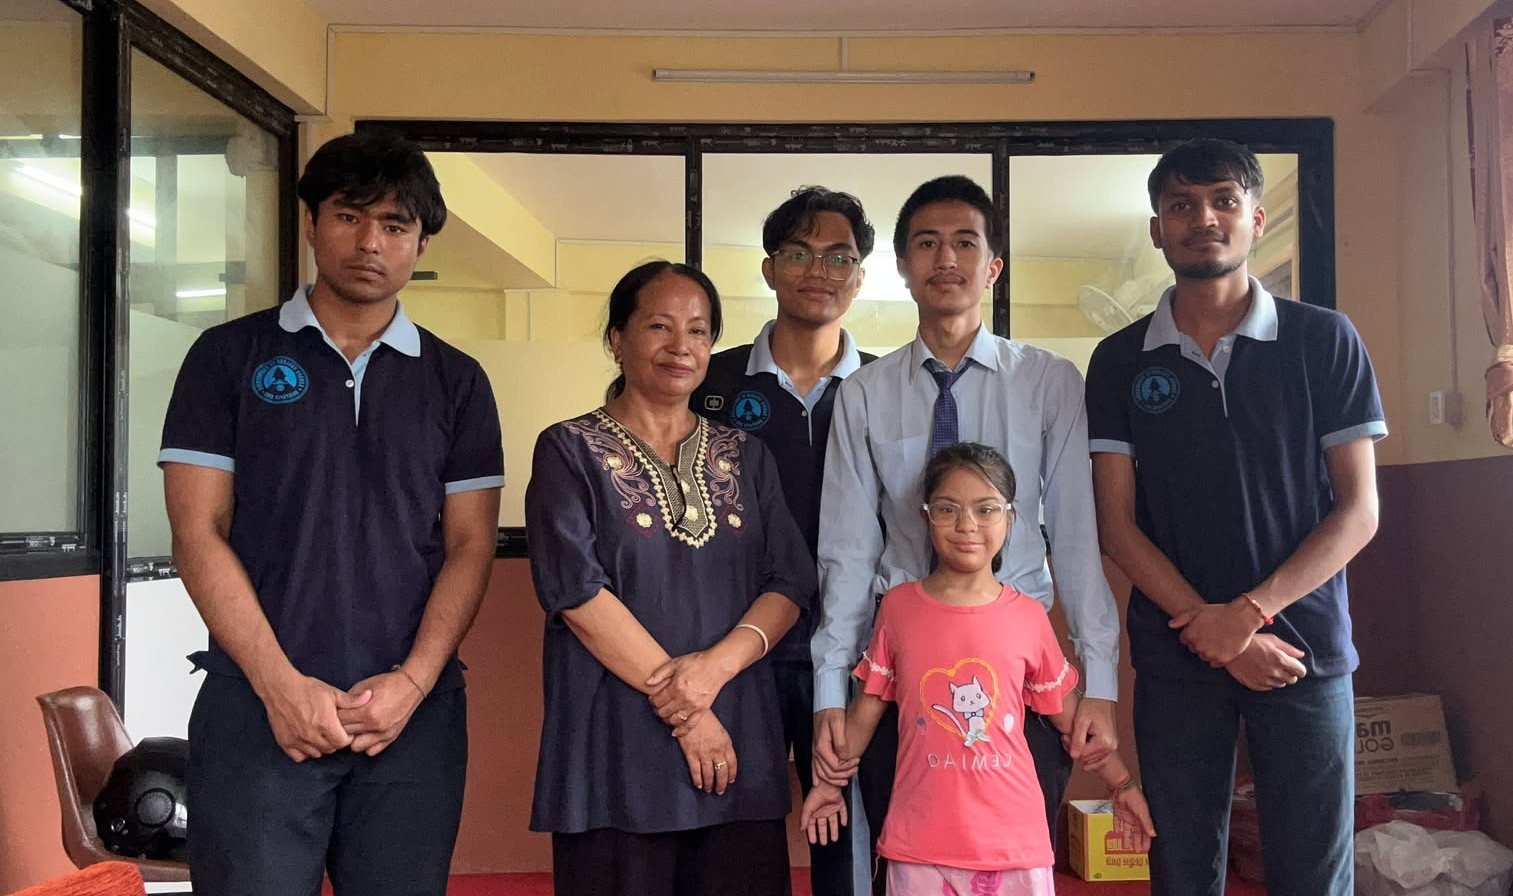
\includegraphics[width=0.72\textwidth]{img/consult1.jpg}
    \caption{The project team with the NSL consultant following a gloss consultation session}
    \label{fig:consult-group}
\end{figure}

\begin{figure}[H]
    \centering
    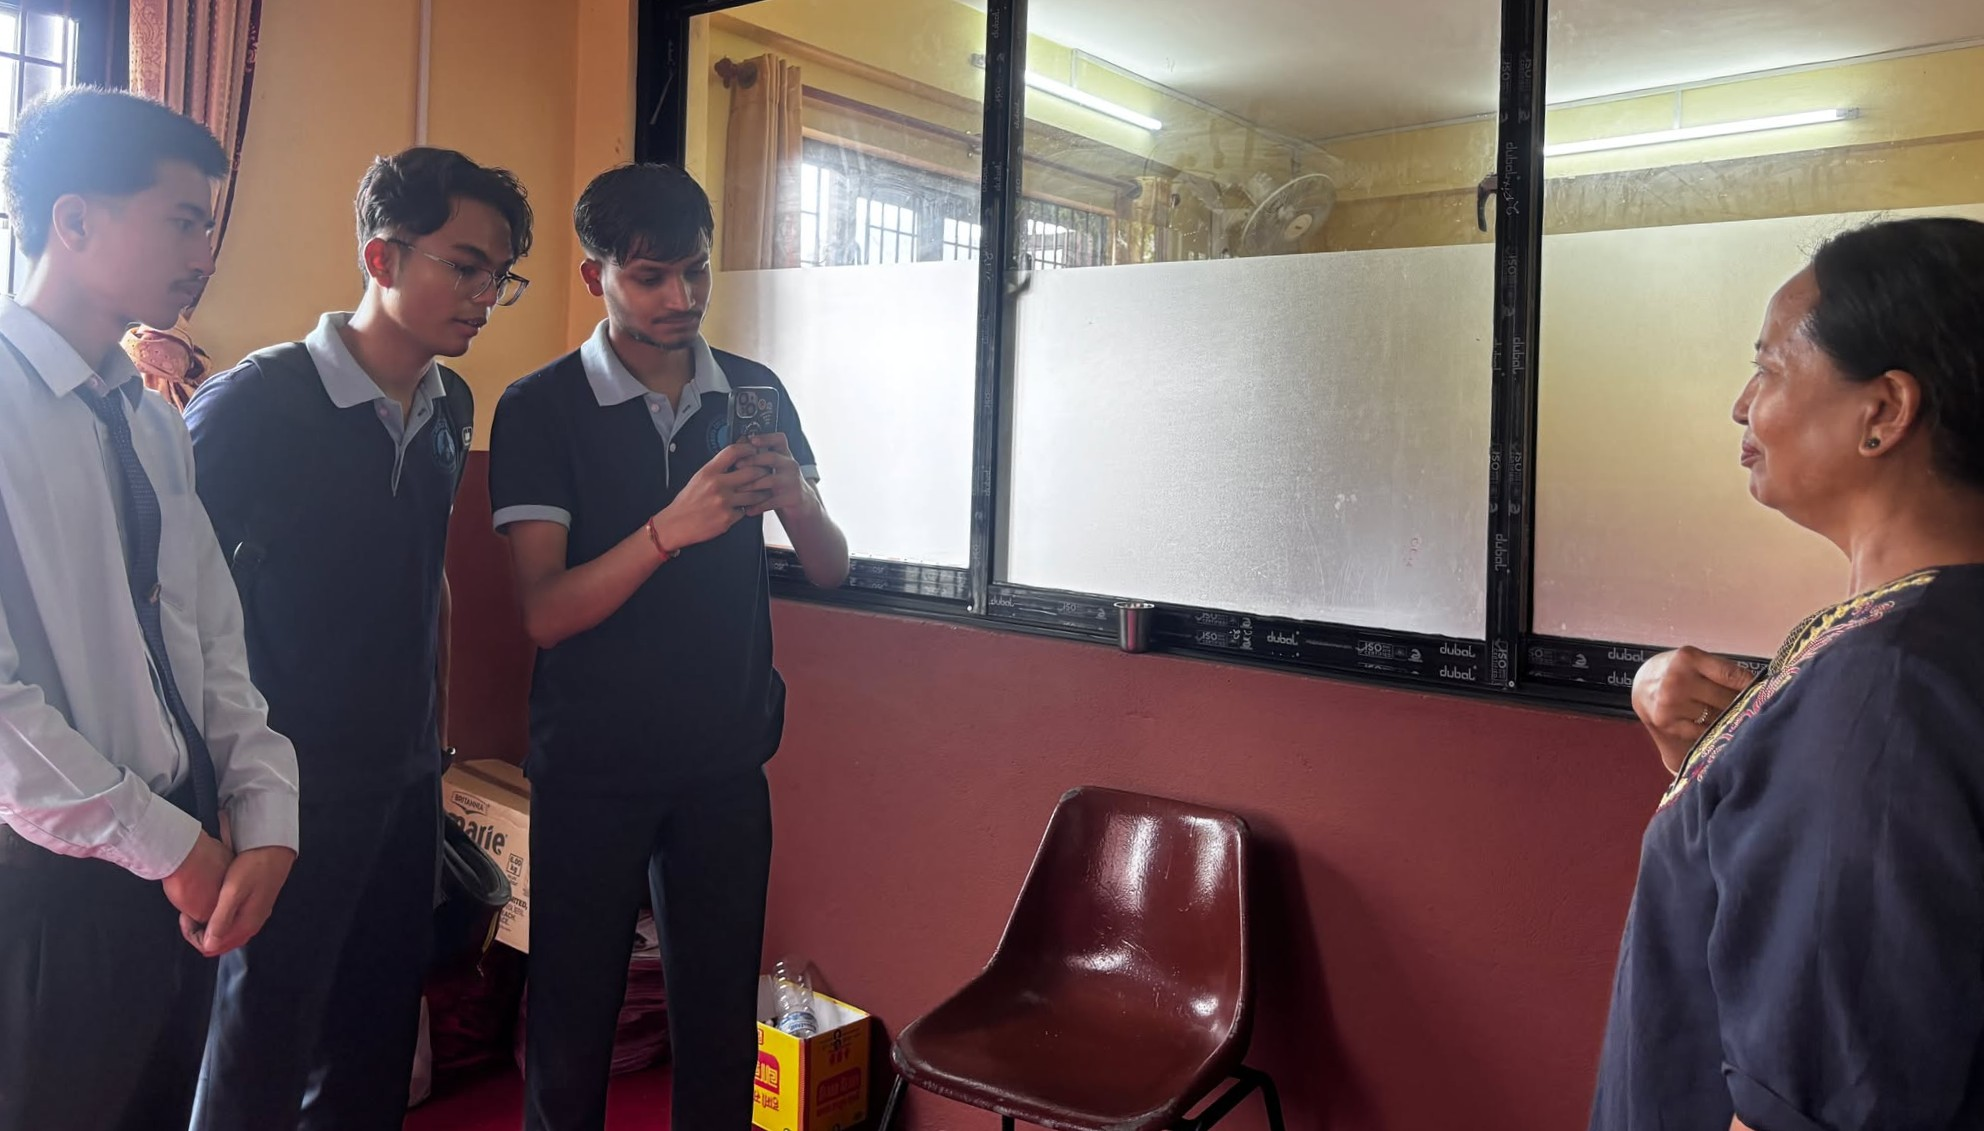
\includegraphics[width=0.72\textwidth]{img/consult2.jpg}
    \caption{Reviewing a recorded demonstration with the consultant to confirm the reference form of a phrase}
    \label{fig:consult-review}
\end{figure}

\begin{figure}[H]
    \centering
    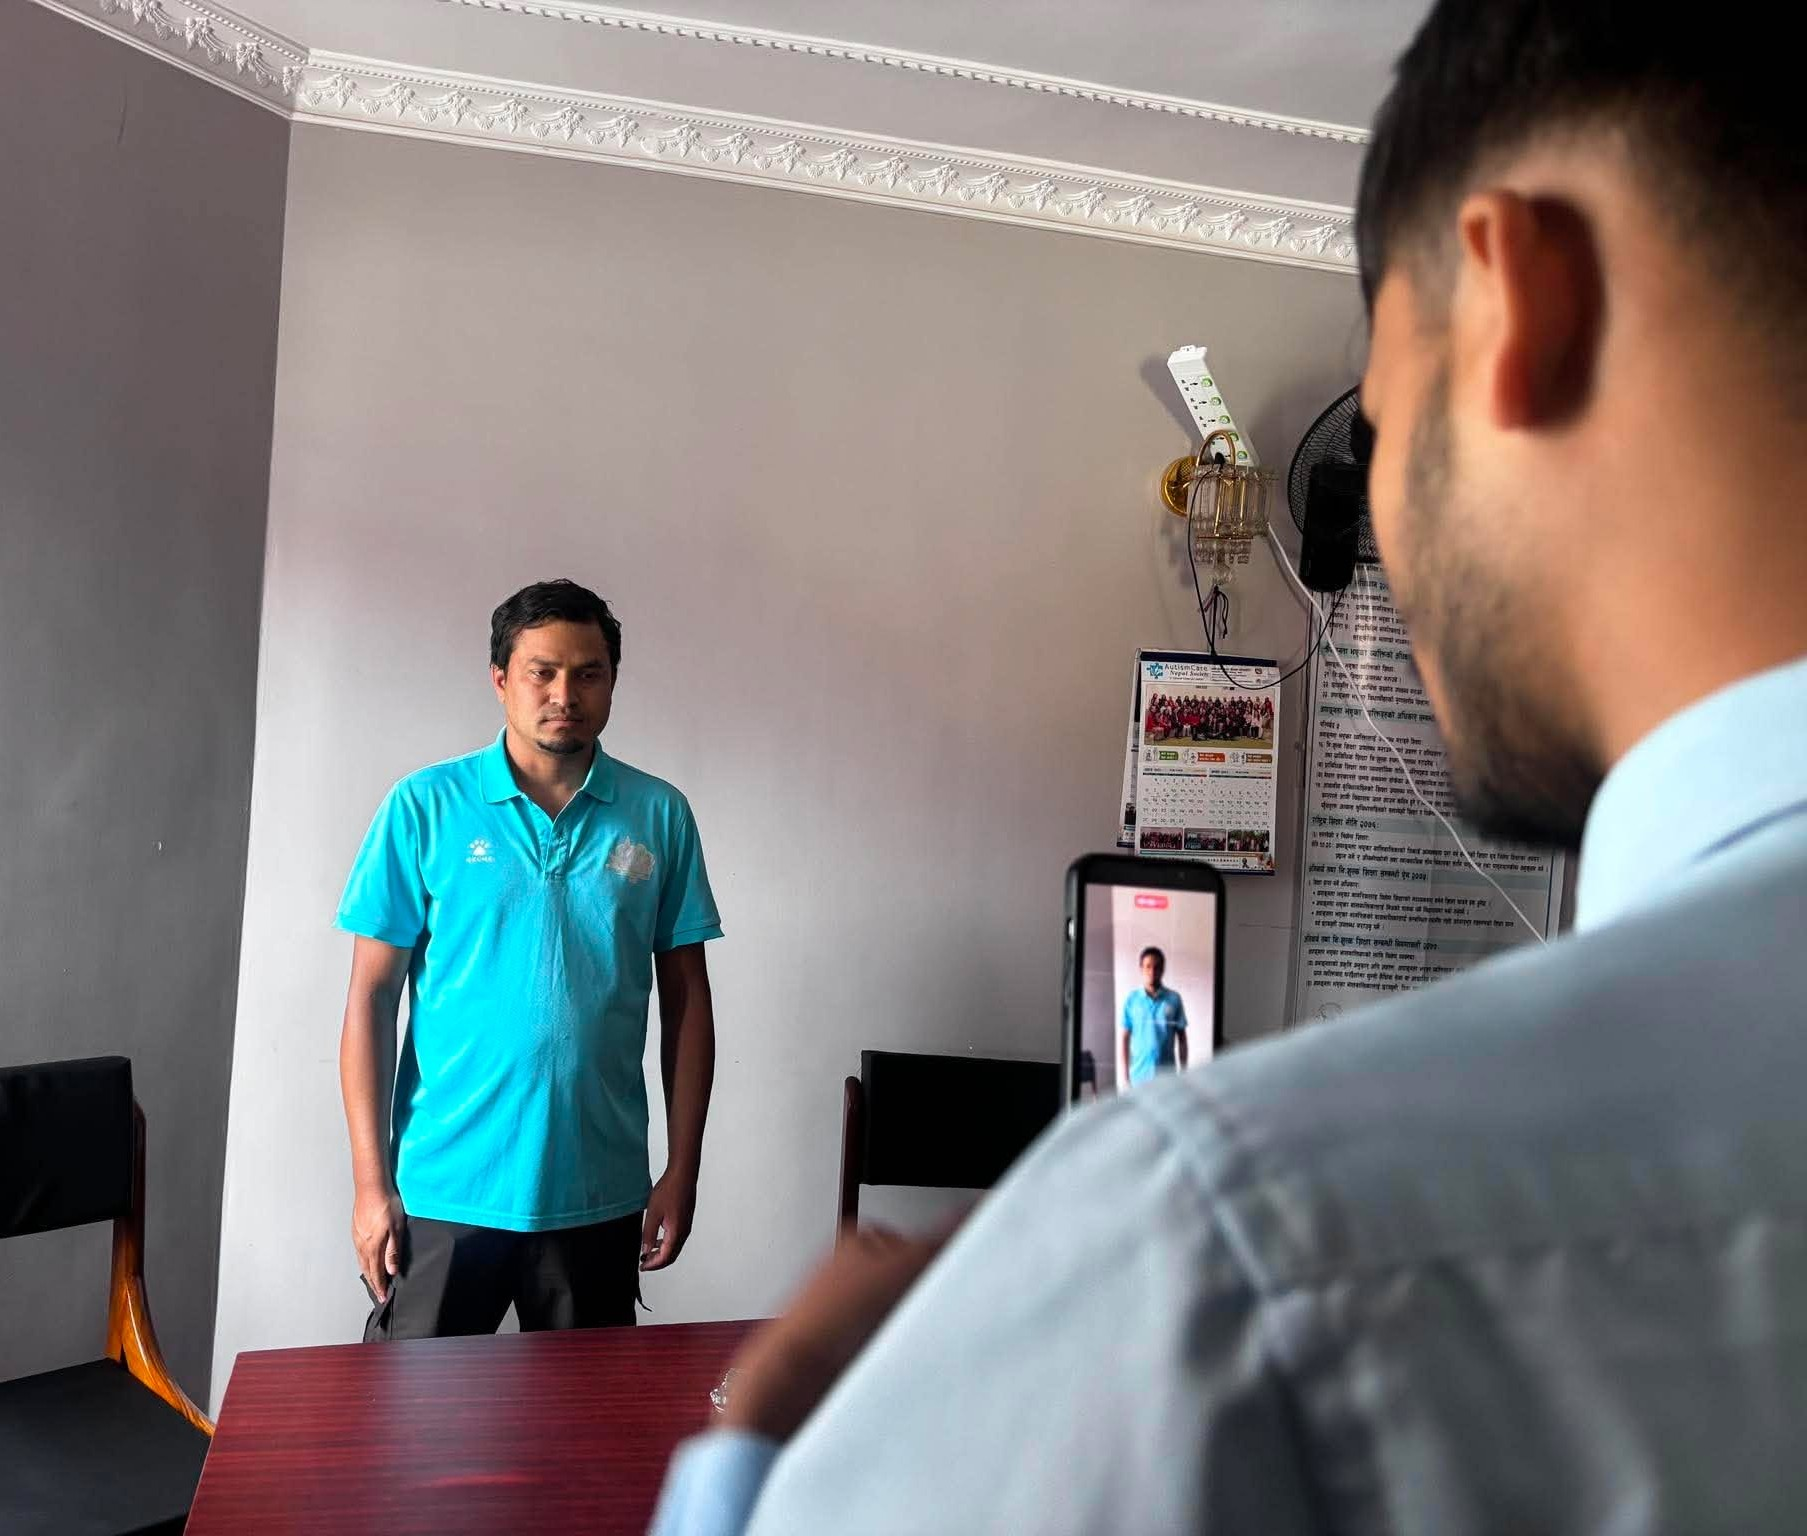
\includegraphics[width=0.72\textwidth]{img/consult3.jpg}
    \caption{An NSL expert demonstrating the signed form of a phrase for reference recording}
    \label{fig:consult-demo}
\end{figure}

% ================= Appendix B =================
\chapter{Data Collection Tool}
\label{app:recorder}

Clips were recorded with a purpose-built tool that runs MediaPipe Holistic on a live webcam feed and saves the 225-value landmark vector for each frame. The operator selects a signer identity and a phrase, then starts and stops each recording explicitly. Landmark overlays are drawn live, so a failed detection is visible during recording instead of afterwards.

\begin{figure}[H]
    \centering
    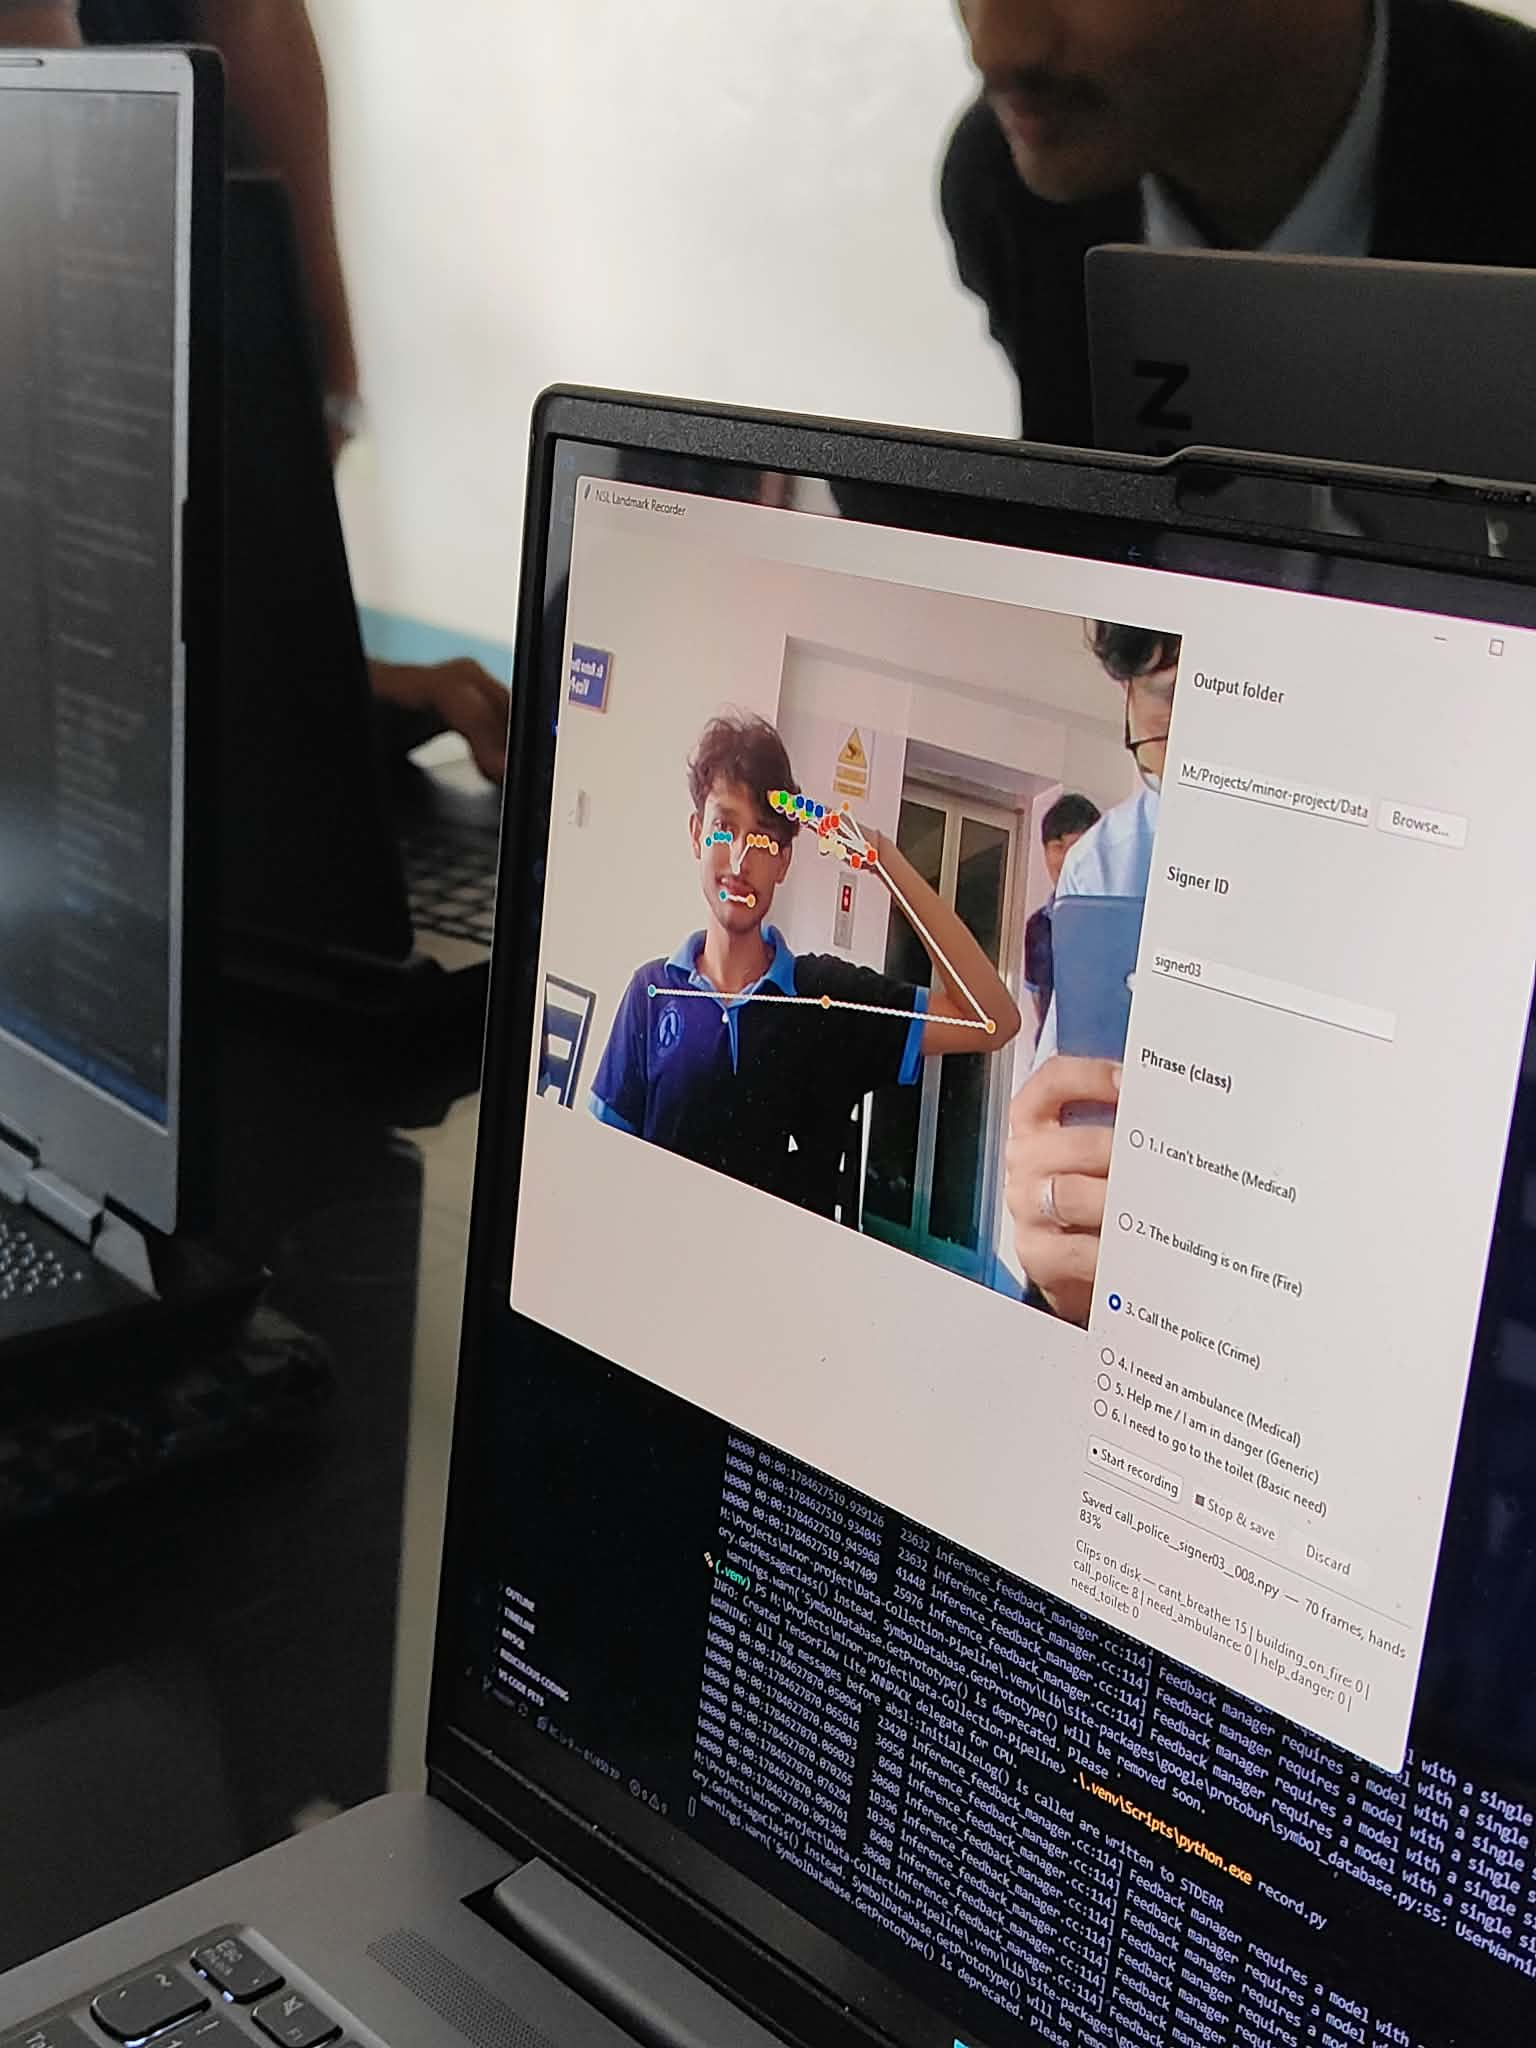
\includegraphics[width=0.88\textwidth]{img/recorder1.jpg}
    \caption{A signer recording the \textit{Call the police} phrase, showing live pose and hand landmark overlays alongside the signer identity and phrase selection}
    \label{fig:recorder-a}
\end{figure}

\begin{figure}[H]
    \centering
    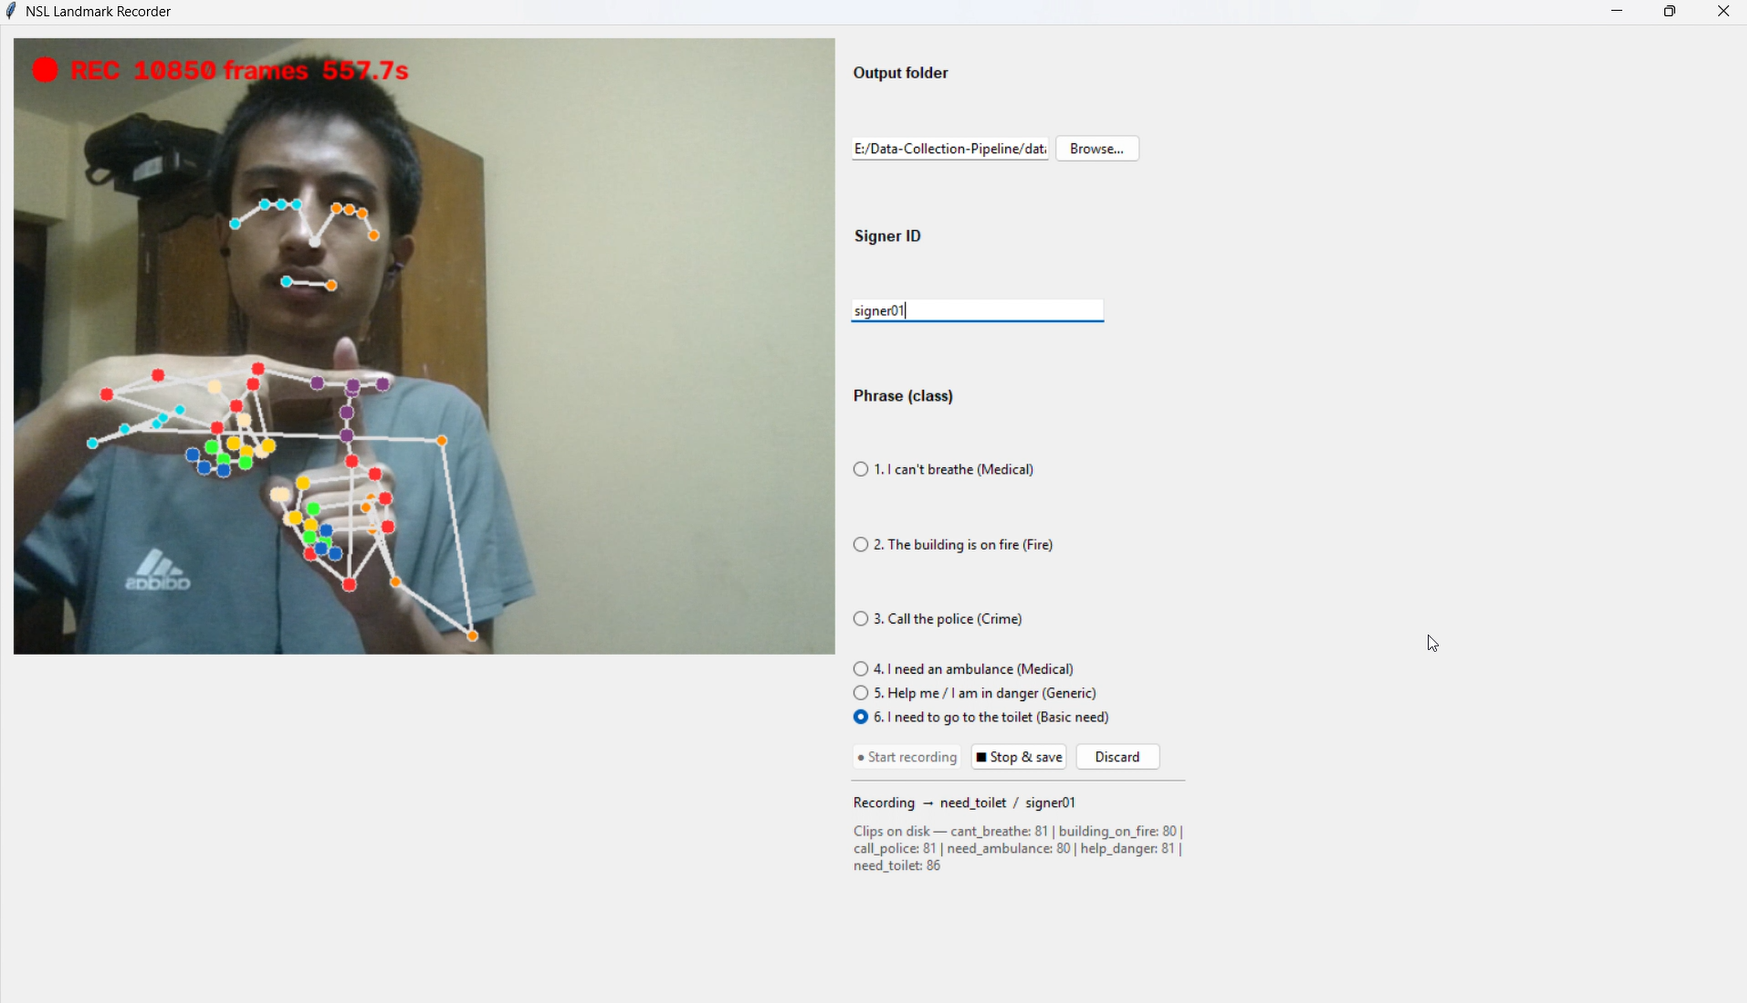
\includegraphics[width=0.88\textwidth]{img/recorder2.png}
    \caption{The recorder during an active recording, showing hand landmarks in detail and the running per-class clip counts on disk}
    \label{fig:recorder-b}
\end{figure}

% ================= Appendix C =================
\chapter{Dataset Organisation}
\label{app:dataorg}

The eight signers recorded independently on separate machines. Contributions were merged through a shared Git repository instead of by hand, which gave a reviewable history of what each signer added and caught duplicate and misnamed clips before they entered the combined dataset.

\begin{figure}[H]
    \centering
    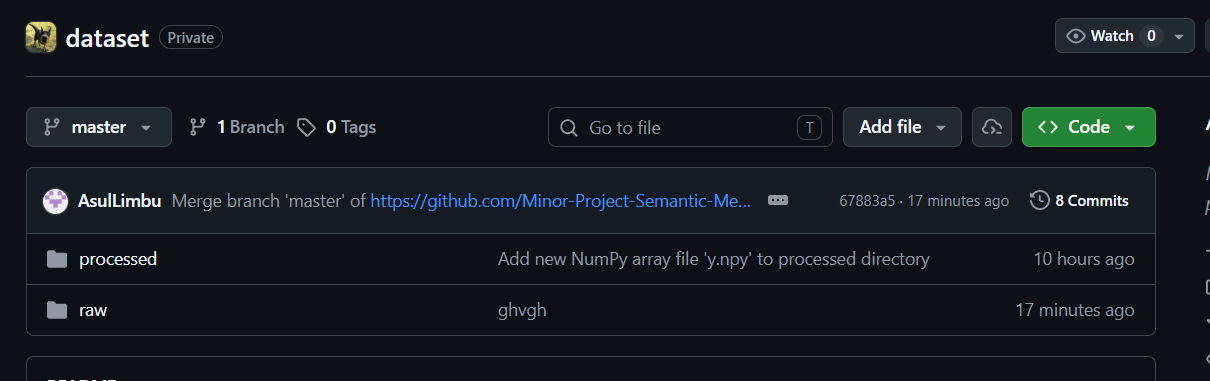
\includegraphics[width=0.88\textwidth]{img/repomerge1.png}
    \caption{The shared dataset repository, with raw and processed directories tracked separately and a commit history showing contributions merged from several signers}
    \label{fig:merge-repo}
\end{figure}

\begin{figure}[H]
    \centering
    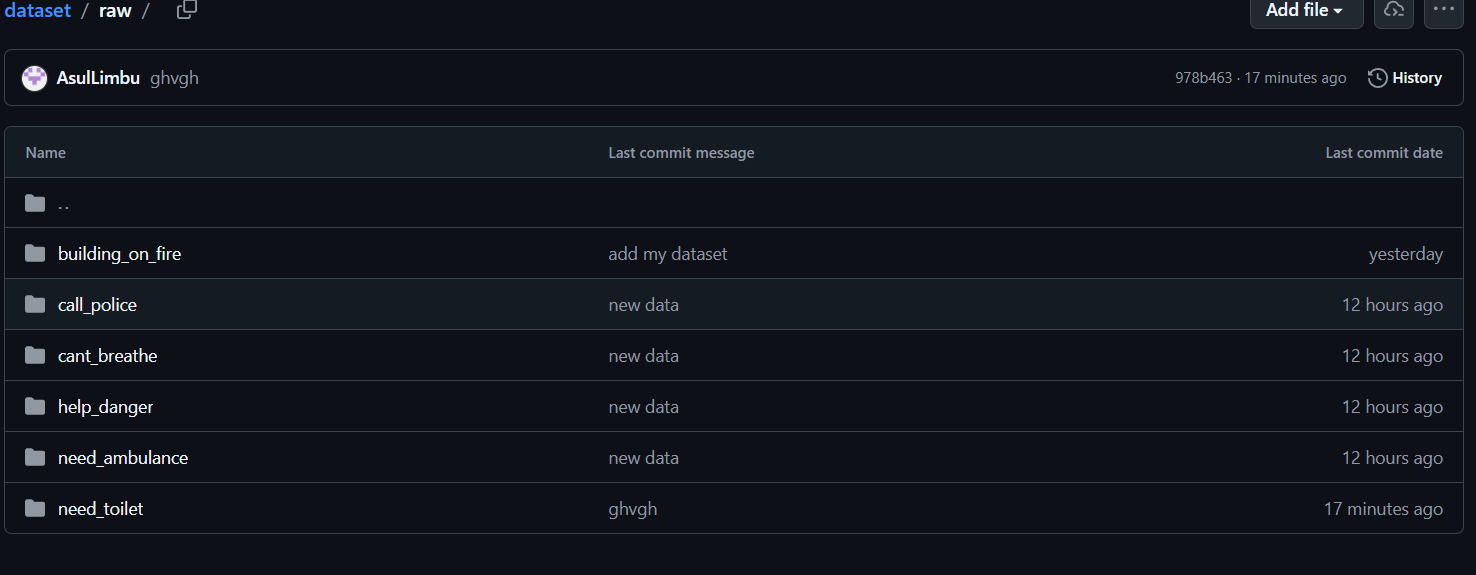
\includegraphics[width=0.88\textwidth]{img/repomerge2.png}
    \caption{The raw directory after merging, with one subfolder per phrase class holding the contributions of all signers}
    \label{fig:merge-raw}
\end{figure}

\begin{figure}[H]
    \centering
    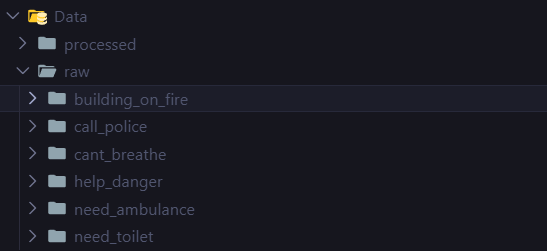
\includegraphics[width=0.5\textwidth]{img/rawdirs.png}
    \caption{Local directory layout: raw clips organised by phrase class, alongside the processed output directory}
    \label{fig:dirs-raw}
\end{figure}

\begin{figure}[H]
    \centering
    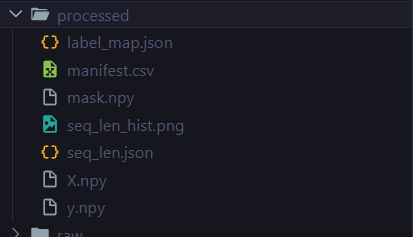
\includegraphics[width=0.42\textwidth]{img/processeddirs.png}
    \caption{Contents of the processed directory: the compiled tensors alongside the manifest and the sequence-length metadata}
    \label{fig:dirs-processed}
\end{figure}

% ================= Appendix D =================
\chapter{Sample Landmark Data}
\label{app:sampledata}

This appendix traces one clip through the preprocessing pipeline, to make the numeric effect of each step concrete. The clip is \texttt{call\_police\_\_signer01\_\_001.npy}, stored as a $(42, 225)$ array of 32-bit floats: 42 recorded frames, each holding one 225-value landmark vector.

\section{Feature Vector Layout}

\begin{table}[H]
    \centering
    \caption{Layout of the 225-value feature vector}
    \label{tab:featurelayout}
    \begin{tabular}{lccl}
        \toprule
        \textbf{Block} & \textbf{Indices} & \textbf{Values} & \textbf{Content} \\
        \midrule
        Pose        & 0 to 98    & 99 & 33 landmarks $\times\ (x, y, z)$ \\
        Left hand   & 99 to 161  & 63 & 21 landmarks $\times\ (x, y, z)$ \\
        Right hand  & 162 to 224 & 63 & 21 landmarks $\times\ (x, y, z)$ \\
        \midrule
        \textbf{Total} & & \textbf{225} & \\
        \bottomrule
    \end{tabular}
\end{table}

\section{Raw Values}

The first five pose landmarks of the clip's first frame, in the normalised image coordinates MediaPipe reports:

\begin{table}[H]
    \centering
    \caption{Raw pose landmarks 0 to 4, first frame}
    \label{tab:rawvalues}
    \begin{tabular}{cccc}
        \toprule
        \textbf{Landmark} & $x$ & $y$ & $z$ \\
        \midrule
        0 & 0.3683 & 0.3315 & $-$1.0291 \\
        1 & 0.3924 & 0.2687 & $-$0.9459 \\
        2 & 0.4069 & 0.2707 & $-$0.9461 \\
        3 & 0.4187 & 0.2732 & $-$0.9460 \\
        4 & 0.3420 & 0.2707 & $-$0.9640 \\
        \bottomrule
    \end{tabular}
\end{table}

\noindent Both hand blocks of this frame are entirely zero. The signer's hands had not yet entered the frame when recording began, MediaPipe reported no hand landmarks, and the recorder filled all 126 values with zeros instead of leaving them undefined.

\section{After Normalisation}

The same five landmarks after dual-anchor normalisation, now expressed relative to the shoulder midpoint and scaled by shoulder width:

\begin{table}[H]
    \centering
    \caption{Normalised pose landmarks 0 to 4, first frame}
    \label{tab:normvalues}
    \begin{tabular}{cccc}
        \toprule
        \textbf{Landmark} & $x$ & $y$ & $z$ \\
        \midrule
        0 & $-$0.0054 & $-$0.7148 & $-$1.6152 \\
        1 & 0.0463 & $-$0.8491 & $-$1.4370 \\
        2 & 0.0772 & $-$0.8449 & $-$1.4374 \\
        3 & 0.1025 & $-$0.8396 & $-$1.4374 \\
        4 & $-$0.0617 & $-$0.8449 & $-$1.4758 \\
        \bottomrule
    \end{tabular}
\end{table}

\noindent The $x$ coordinates now sit around zero instead of around 0.37, because the origin has moved to the midpoint of the shoulders. The zero hand blocks remain exactly zero, since both normalisation formulas map a zero input to a zero output.

\section{After Length Standardisation}

The clip has 42 frames, fewer than the sequence length of 146, so it is zero-padded at the end. The result is a $(146, 225)$ array in which the first 42 frames are real and the remaining 104 are zero, with a boolean mask recording which is which. The final frame of the standardised clip is entirely zero, confirming that padding stays distinguishable from signal and that the masking layer will skip it.

% ================= Appendix E =================
\chapter{Client Interface}
\label{app:ui}

The Android client presents one of two outcomes for every recognition attempt: an accepted phrase, which is displayed and spoken, or a low-confidence result, which is reported without being spoken. A row of indicators below the camera preview reports what the server observed for each frame, so a failure during use can be attributed instead of guessed at.

\fillin{Insert client screenshots here: the accepted and low-confidence result states, the telemetry indicator row, and the server configuration screen.}

% ================= Appendix F =================
\chapter{Server Interface}
\label{app:protocol}

The inference server exposes the endpoints in Table~\ref{tab:endpoints}. The streaming endpoint is the path the client uses; the two prediction endpoints exist so that the server can be checked against the offline pipeline without needing a phone.

\begin{table}[H]
    \centering
    \caption{Server endpoints}
    \label{tab:endpoints}
    \small
    \begin{tabular}{|l|l|c|p{6.1cm}|}
        \hline
        \textbf{Method} & \textbf{Path} & \textbf{Key} & \textbf{Purpose} \\
        \hline
        GET  & \texttt{/health}            & no  & Backend, class list, thresholds, target frame rate \\
        \hline
        GET  & \texttt{/classes}           & yes & Class keys and display labels \\
        \hline
        POST & \texttt{/predict/landmarks} & yes & A clip supplied as JSON, for verification \\
        \hline
        POST & \texttt{/predict/npy}       & yes & The same clip as raw array bytes \\
        \hline
        WS   & \texttt{/ws/stream}         & yes & Live frames to a decision, the path the client uses \\
        \hline
    \end{tabular}
\end{table}

\noindent The health endpoint is deliberately unauthenticated so that container health checks and the client's reachability test keep working when a key is configured. Every other endpoint requires the key, compared with a constant-time function so that a wrong key cannot be narrowed down by timing the response.

\begin{table}[H]
    \centering
    \caption{Messages on the streaming endpoint}
    \label{tab:wsmessages}
    \small
    \begin{tabular}{|l|l|p{7.3cm}|}
        \hline
        \textbf{Direction} & \textbf{Message} & \textbf{Meaning} \\
        \hline
        Server & \texttt{ready}     & Session established; carries the target frame rate and class list \\
        \hline
        Client & binary frame       & One JPEG frame \\
        \hline
        Server & \texttt{ack}       & Whether the frame was kept, the running frame count, and whether pose and hands were detected \\
        \hline
        Client & \texttt{done}      & Signing has finished; produce a decision \\
        \hline
        Server & \texttt{result}    & Status, phrase, confidence, and the three most probable classes \\
        \hline
        Client & \texttt{reset}     & Discard the current clip and start again \\
        \hline
        Client & \texttt{ping}      & Keepalive, sent while idle between signs \\
        \hline
    \end{tabular}
\end{table}
